% File: traffic_control_signals.tex, author: John Sauter,
% date: November 27, 2025.

% Copyright © 2025 by John Sauter.
% Licensed under the Creative Commons Attribution-ShareAlike 4.0 International
% license.  See https://creativecommons.org/license/by-sa/4.0/.

\documentclass[letterpaper,twoside]{article}
\usepackage[capbesideposition=outside,facing=no,capbesidesep=quad]{floatrow}
\usepackage{fontspec}
\usepackage{lmodern}
\usepackage{amsmath}
%\usepackage[english]{babel}
\usepackage{xcolor}
%\usepackage{multicol}
\usepackage{array}
\usepackage{longtable}
\usepackage{enumitem}
\usepackage[super]{nth}
\usepackage{fancyhdr}
\usepackage{xfrac}
\usepackage{fnpct}
\usepackage{siunitx}
\usepackage{graphicx}
\usepackage{natbib}
\usepackage[kpsewhich=true]{minted}
\usepackage[tracking]{microtype}
\usepackage{hyphenat}
\usepackage{fancyvrb}
\usepackage{relsize}
\usepackage{hyperxmp}
%\usepackage{flexisym}
\usepackage{media9}
\usepackage{tikz}
\usetikzlibrary {babel}

% Font choices: pick one.

% 1. Latin Modern matches Don Knuth's Computer Modern
% Note that Latin Modern displays U+02BC (Modifier Letter Apostrophe)
% as a space.  This letter is used when naming Mesoamerican
% Long Count dates.
%\usepackage{unicode-math}
%\setmainfont{Latin Modern Roman}[SmallCapsFont={Latin Modern Roman Caps}]
%\setmonofont{Latin Modern Mono}
%\setmathfont{Latin Modern Math}
%\newcommand{\filename}{\ttfamily\smaller}

% 2. Libertine
%\usepackage{unicode-math}
%\setmainfont[Ligatures={Common},Numbers=Proportional]{Linux Libertine O}
%\setsansfont{Linux Biolinum O}
%\setmathfont[Scale=MatchUppercase]{libertinusmath-regular.otf}
%\newcommand{\filename}{\ttfamily}

% 3. Garamond Libre
%\usepackage{unicode-math}
%\usepackage{garamondlibre}
%\newcommand{\filename}{\ttfamily}

% 4. Old Standard
% Small caps doesn't work.
%\usepackage{unicode-math}
%\setmainfont{OldStandard}
%\newcommand{\filename}{\ttfamily}

% 5. Liberation
% Small caps doesn't work.
%\usepackage{unicode-math}
%\defaultfontfeatures{Scale=MatchLowercase}
%\setmainfont{Liberation Serif}
%\setsansfont{Liberation Sans}
%\setmonofont[SmallCapsFont={Liberation Mono}]{Liberation Mono}
%\newcommand{\filename}{\ttfamily}

% 6. GNU Freefont
%\usepackage{unicode-math}
%\setmainfont{FreeSerif}
%\setsansfont{FreeSans}
%\setmonofont{FreeMono}
%\newcommand{\filename}{\ttfamily\smaller}
%\renewcommand\RSpercentTolerance{0}

% 7. Andika
%\usepackage{unicode-math}
%\setmainfont{Andika}
%\newcommand{\filename}{\ttfamily}

% 8. Bahnschrift
%\usepackage{unicode-math}
%\setmainfont{Bahnschrift}
%\newcommand{\filename}{\ttfamily}

% 9. Charis Sil
%\usepackage{unicode-math}
%\setmainfont{Charis Sil}
%\newcommand{\filename}{\ttfamily}

% 10. E B Garamond
%\usepackage{unicode-math}
%\setmainfont{ebgaramond}
%\setsansfont{Charis Sil}
%\setmonofont[SmallCapsFont={Liberation Mono}]{source code pro}
%\setmathfont{Garamond-Math.otf}
%\newcommand{\filename}{\ttfamily\smaller}

% 11. Junicodevf, not yet available in TexLive-2023/Fedora 40 as of
% June 30, 2024.
%\usepackage{unicode-math}
%\usepackage[
%  MainRegularSizeFeatures={
%    {size=8.6,wght=550,wdth=120},
%    {size=10.99,wght=475,wdth=115},
%    {size=21.59,wght=400,wdth=112.5},
%    {size=21.59,wght=351,wdth=100}
%  },
%  MainItalicSizeFeatures={
%    {size=8.6,wght=550,wdth=118},
%    {size=10.99,wght=475,wdth=114},
%    {size=21.59,wght=450,wdth=111},
%    {size=21.59,wght=372,wdth=98}
%  },
%  MainBoldSizeFeatures={
%    {size=8.6,wght=700,wdth=120},
%    {size=10.99,wght=700,wdth=115},
%    {size=21.59,wght=650,wdth=112.5},
%    {size=21.59,wght=600,wdth=100}
%  },
%  MainBoldItalicSizeFeatures={
%    {size=8.6,wght=700,wdth=118},
%    {size=10.99,wght=700,wdth=114},
%    {size=21.59,wght=650,wdth=111},
%    {size=21.59,wght=600,wdth=98}
%  }
%]{junicodevf}
%\newcommand{\filename}{\ttfamily\smaller}

% 12. Lato, not yet available in TexLive-2023/Fedora 40 as of June 1, 2024
%\usepackage[default]{lato}
%\usepackage[default]{lete-sans-math}
%\setsansfont{Lato}[Extension = .ttf,
%  UprigthtFont = *-Regular,
%  BoldFont = *-Bold,
%  ItalicFont = *-Italic,
%  BoldItalicFont = *-BoldItalic]
%\newcommand{\filename}{\ttfamily\smaller}

% 13. New Computer Modern, book weight
\usepackage{unicode-math}
\usepackage{newcomputermodern}
\newcommand{\filename}{\ttfamily\smaller}

\usepackage[pdfencoding=unicode,pagebackref,breaklinks]{hyperref}
\bibliographystyle{plainnat}
\setcitestyle{numbers,square}
% Pages styles
%\setlength{\headheight}{22.5pt}
\pagestyle{fancy}
\fancyhead{}
\fancyhead[LE]{\thepage}
\fancyhead[CE]{{\scshape John Sauter}}
\fancyhead[CO]{{\scshape how traffic control signals work}}
\fancyhead[RO]{\thepage}
\renewcommand{\headrulewidth}{0pt}
\fancyfoot{}
\setlength\tabcolsep{1mm}
\renewcommand\arraystretch{1.3}

\begin{document}
\title{How Traffic Control Signals Work\footnote{Copyright
    {\copyright} 2025 by John Sauter.
    This paper is made available under a
    Creative Commons Attribution-ShareAlike 4.0 International License.
    You can read a human-readable summary of the license at
    \href{https://creativecommons.org/licenses/by-sa/4.0}{https://creativecommons.org/licenses/by-sa/4.0},
    which contains a link to the full text of the license.
    See also section \ref{section:Licensing} of this paper.}
}
\author{John Sauter\footnote{
    System Eyes Computer Store,
    20A Northwest Blvd.  Ste 345,
    Nashua, NH  03063-4066,
    e-mail: John\_Sauter@systemeyescomputerstore.com,
    telephone: (603) 424-1188}}
\hypersetup{unicode=true,
  pdfauthor={John Sauter},
  pdftitle={How Traffic Control Signals Work},
  pdfsubject={traffic control signals},
  pdfkeywords={traffic intersections signals},
  pdfcontactaddress={System Eyes Computer Store, 20A Northwest Blvd.  Ste 345},
  pdfcontactcity={Nashua},
  pdfcontactcountry={USA},
  pdfcontactemail={John\_Sauter@systemeyescomputerstore.com},
  pdfcontactphone={603-424-1188},
  pdfcontactpostcode={03063-4066},
  pdfcontactregion={New Hampshire},
  pdfcontacturl={https://www.systemeyescomputerstore.com},
  pdfcopyright={Copyright {\copyright} 2025 by John Sauter},
  pdfurl={https://www.systemeyescomputerstore.com/How\%5FTraffic\%5FControl\%5FSignals\%5fWork/traffic\%5Fcontrol\%5Fsignals.pdf},
  pdfdate={2025-11-27},
  pdflicenseurl={https://creativecommons.org/licenses/by-sa/4.0},
  pdfmetalang={en-US}
}

\date{2025-11-27}
\maketitle
\begin{abstract}
  Traffic control signals allow vehicles and pedestrians to move through
  intersections safely and efficiently.  Here is how they work.
\end{abstract}
\begin{description}
\item[Keywords:]traffic control signals; traffic intersections; traffic.
\item[URL:]\href{https://www.systemeyescomputerstore.com/How\_Traffic\_Control\_Signals\_Work/traffic\_control\_signals.pdf}{https://www.systemeyescomputerstore.com/How\_Traffic\_Control\_Signals\_Work/traffic\_control\_signals.pdf}
\end{description}
%\tableofcontents
\newpage

\section{Introduction}
At a traffic intersection vehicles and pedestrians must cross each other's
path.  To allow this to happen safely, a traffic control signal is used to
delay traffic in one direction while it proceeds in another.  To maximize
efficiency, the traffic control signal lets traffic flow when there is a
long line of vehicles and allows multiple traffic flows provided they
do not intersect.  However, making a vehicle wait too long compromises safety,
since a vehicle operator will consider an excessive  delay as an indication
that the traffic control signal is not working, and proceed into the
intersection in spite of it.

In the United States, the standard for traffic control devices is the
Manual on Uniform Traffic Control Devices, known as MUTCD\citep{MUTCD11}.
Much of the terminology and some of the pictures
in this paper were taken from that document.

We describe a traffic control signal as a set of finite state machines,
one for each lane that provides entry to the intersection.
A finite state machine is a process within a computer which has
a limited number of states that it can be in, and for each state
there are rules for making a transition to another state.
Each finite state machine is associated with an entry lane
and controls the signal face which is displayed to traffic
entering the intersection through that lane.  A lane's finite
state machine has timers and toggles so it can communicate
with the environment, as described below.

\section{Example 01: Single-lane Bridge}

To describe how traffic control signals work we begin with a simple
example: a single-lane bridge:

\begin{figure}[htb]
  {\includegraphics[width=\textwidth]{background_01}}
  {\caption{Example 01: single-lane bridge}\label{fig:single-lane_bridge}}
\end{figure}

In figure \ref{fig:single-lane_bridge} vehicles approach from the west
on lane A.  From there they can cross the bridge and exit on lane 1,
or make a U-turn and exit on lane 2.  Similarly, vehicles approach
from the east on lane B and either cross the bridge, exiting on lane 2,
or make a U-turn and exit on lane 1.

\subsection{Conflicts}

We need to examine the intersection to see where, when traffic is moving
in one way, it must not be permitted to move in another way.  We call each
way that vehicles can move a travel path, and each travel path is named
for the entering and exiting lane.  Here we have travel paths A1, A2, B1,
and B2.  The two U-turns, A2 and B1, do not interfere with each other, but
A1 conflicts with B2 and B2 conflicts with A1 since they place two vehicles
on the one-lane bridge going in opposite directions.

When a vehicle reaches the bridge on lane A or B we do not
know which lane it intends to exit on, so we must block all travel paths
which conflict with any travel path starting at that lane.  Thus,
lane A must be blocked when a vehicle has entered the bridge from lane B,
and vice-versa.

This conflict analysis is simple for the one-lane bridge but as we will see
later it is more complex for complex intersections.

\subsection{Signal Faces}

In order to allow vehicles to cross the bridge safely, we need signal
faces on lanes A and B to stop traffic from entering the bridge if
traffic is moving the other way.

A signal face looks like this:

\begin{figure}[H]
  \fcapside[\FBwidth]
           {\includegraphics*{signal_ccc}}
           {\caption{signal face with three circular lamps}
             \label{fig:signal_ccc}}
\end{figure}

Vehicle operators know that if the red lamp is lit they may not
enter the intersection.  The green lamp allows the vehicle to
proceed, and the yellow lamp gives warning that the red lamp
is about to light.

For maximum efficiency, whenever possible a vehicle approaching
a signal face should see a green light so it doesn't have to
stop or even slow down as it crosses the bridge.  To make this
work from both directions we need to keep both signal faces red
until a vehicle approaches, then turn that lane's signal face
green.

\subsection{Sensors}

The finite state machine associated with a lane needs to know
what traffic is flowing through that lane so it can set its
signal face appropriately.  This information is provided
by vehicle sensors buried under the roadway.
When a vehicle passes over a sensor we say that the sensor
has been triggered.

\subsubsection{Traffic Present}

Lanes A and B each have a vehicle sensor at the stop line where the lane
meets the intersection.  This sensor tells the finite state machine
that a vehicle is entering the intersection or is waiting to enter.
We call this the Traffic Present sensor.

\subsubsection{Traffic Approaching}

For safety reasons the Traffic Present sensor isn't sufficient.
Because bridge traffic is very light, vehicle operators will be
used to seeing the signal face turn green when they reach
the intersection, and when it doesn't they will be unable to stop
before entering the bridge.  To solve this problem we need a
second vehicle sensor set back from the Traffic Present sensor.
This lets the finite state machine turn the signal face green
before the vehicle is
close to the intersection.  If the vehicle operator does not
see the green light when he is used to seeing it he will have
time to stop safely.  We call this the Traffic Approaching sensor.

\subsection{Timers}

In addition to the lane's signal face and sensors, the
finite state machine needs a sense of time.  Here are the most
important timers:

\subsubsection{Red Clearance Time}
The Red Clearance time is the time between when a signal face turns red
and the last vehicle to enter the bridge from that lane has left the
bridge, so that we can give the other lane a green light.

\subsubsection{Yellow Change Time}
To give traffic warning that the finite state machine will soon
set the signal face to red it first turns the signal face yellow
for Yellow Change time.

\subsubsection{Minimum Green Time}
After turning a signal face green the finite state machine
gives the traffic this much time to get moving before it considers
turning the signal face red.

\subsubsection{Passage Time}
When a vehicle operator sees a signal face turn yellow, he must stop
before entering the intersection if he can do so safely, or proceed
through the intersection if he cannot.  This decision is easy to make
if the vehicle is close to the intersection or far from it, but is hard
to make in an intermediate situation.  To avoid this, the finite state
machine tries to turn the signal face yellow only when there are no
vehicles in this intermediate situation.

The finite state machine does this by monitoring the Traffic Approaching
sensor.  If no vehicle has activated this sensor for Passage Time seconds,
the finite state machine can be sure that any vehicles are either so close
to the intersection that they can safely make it through before the signal
face turns red, or far enough away that they clearly cannot.
We call this a gap in the traffic.

\subsubsection{Maximum Green time}
If the finite state machine has been looking for a gap in the traffic
in order to turn red for Maximum Green time seconds, it turns red
anyway.  This will allow cross traffic to proceed even when it needs
to stop a line of continuous traffic.

\subsubsection{Green Limit Time}

If the signal face has been green for Green Limit seconds, the finite state
machine will set the signal face to red even if there is no conflicting
traffic and there is traffic passing through this finite state machine's lane.

\subsubsection{Red Limit Time}
If the signal face has been red for this many seconds, the finite state
machine will set the signal face to green even if there is no traffic.

\subsection{Timer Durations}

Here are the lengths of time that each timer runs:

\newcolumntype{P}[1]{>{\centering\arraybackslash}p{#1}}
\newcolumntype{M}[1]{>{\centering\arraybackslash}m{#1}}
\newcolumntype{L}{>{\centering\arraybackslash}l}

\input {timer_durations_01.tex}

\subsection{Toggles}

When a finite state machine detects a vehicle approaching it must not turn
its signal face green if there is a vehicle already on the bridge coming
the other way.
This means that the finite state machines must communicate with each other.
They do this with toggles.  Toggles are also used to tell the finite
state machines that their sensors have been triggered.

A toggle may be either set (true) or clear (false).
Here are the most important toggles:

\subsubsection{Traffic Approaching}

When a lane's Traffic Approaching sensor has detected a vehicle
it sets this toggle in the lane's finite state machine.
The toggle remains set after the sensor is no longer
detecting a vehicle until it is cleared by the finite state machine.

\subsubsection{Traffic Present}

When a lane's Traffic Present sensor has detected a vehicle
it sets this toggle in the lane's finite state machine.
The toggle remains set after the sensor is no longer
detecting a vehicle until it is cleared by the finite state machine.

\subsubsection{Request Green}

When a finite state machine's signal face is red but
the finite state machine wants to turn it green it set this toggle.

\subsubsection{Green Request Granted}

When a finite state machine sees this toggle set it can ask the conflicting
finite state machines to block their lane's traffic.

\subsubsection{Request Partial Clearance}

When a finite state machine has been granted its request to turn
its signal face green it sets
the Request Partial Clearance toggle.  This causes the Clearance Requested
toggle to be set in the other finite state machines which control lanes
that conflict with this one.  In this example, if finite state machine
A sets its Request Partial Clearance toggle, that will cause the
Clearance Requested toggle to be set in finite machine B, and vice versa.

\subsubsection{Clearance Requested}

When the other finite state machines see that their Clearance Requested
toggles have been set, they start the process which will lead to
them turning their signal faces red.

\subsubsection{Cleared}

When a finite state machine's signal face has been red long enough for all
of the traffic which entered the intersection through this finite state
machine's lane to have cleared the intersection the finite state machine
sets its Cleared toggle.
This causes the Conflicting Paths are Clear toggle to be set
in finite state machines which are waiting for it.

\subsubsection{Conflicting Paths are Clear}

When a finite state machine sees this toggle set it can change its signal
face from from red to green.

\subsubsection{Traffic Flowing}

When a finite state machine has turned its signal face green it sets the
Traffic Flowing toggle to indicate that it no longer needs to turn
its signal face green.
Doing this gives permission to the other finite state machine to begin the
process of turning its signal face green, when and if it needs to.

\subsection{Wiring the Finite State Machines to the Lamps}

Each finite state machine is wired to the signal face lamps in the
signal face that it controls.
Table \ref{lamp_map_01} shows wiring between the signal
face finite state machines and the lamps in their signal faces.
The mapping is simple for this example but is more complex
for the examples we will discuss later.

\input {lamp_map_names_01.tex}

\subsection{Wiring the Finite State Machines to the Sensors}

Each finite state machine is wired to the sensors
for its lane.  Again, the mapping is simple for this example
but will be more complex later.

\input {sensor_map_01.tex}

\subsection{Process}

With these resources we can construct a process which uses them
to move traffic safely and efficiently across the bridge.
We have two finite state machines, one for each signal face,
and some system programs to let them communicate using toggles.

Here are the states for each finite state machine.  Each state
has substates which we will ignore for now.

\subsubsection{Red State}
When a finite state machine is in the red state its signal face is red.
If it has been in the red state for Red Clearance Time seconds
it sets the Cleared toggle.

If it sees that the Traffic Approaching toggle is set it sets
the Request Green toggle, which will eventually lead to it moving
to the green state.

\subsubsection{Yellow State}
When a finite state machine is in the yellow state its signal face is yellow.
If it has been in the yellow state for Yellow Change Time seconds it moves
to the red state.

\subsubsection{Green State}
When a finite state machine is in the green state its signal face is green.
If it sees that the Clearance Requested toggle is set it moves to the
yellow state when there is a gap in the traffic, or if too much time
passes without a gap.

\subsubsection{System Programs}

The green request granted system program looks for the Green Request
toggle in either finite state machine and sets that finite state machine's
Green Request Granted toggle.
Other system programs mediate the other stages of moving the
finite state machines between states.  These system programs act
in a more complex way when the intersection is more complex.

\subsection{Illustrations}

\subsubsection{Idle}

When the intersection starts up all toggles are set to false,
all timers are set to stopped, and each finite state machine
is set to state Red.
Because the Red Limit timers have infinite duration both finite state machines
will remain red until some traffic appears.

Here is the detailed log:

\input{idle_01_table.tex}

\subsubsection{Single Car}

Consider a single car approaching the bridge from the west.

\noindent\includemedia[width=\textwidth,
  addresource=bridge_one_car_animation_01.mkv,
  activate=onclick, attachfiles,
  flashvars={source=bridge_one_car_animation_01.mkv &loop=false}
]{{\includegraphics[width=\textwidth]{background_01}}}{VPlayer.swf}

In the above animation, the car coming from the west activates the Traffic
Approaching sensor for lane A.  The signal face for lane B has been red
for some time so signal face A immediately turns green.  The car passes
across the bridge without stopping after which signal face A turns
back to red.

If your PDF viewer will not play the animation you can see it on Youtube
by navigating to URL \href%
{https://www.youtube.com/playlist?list=PLCGHQeqDmNySa8JSIUioGNoWbXebCGjyx}%
{https://www.youtube.com/playlist?list=PLCGHQeqDmNySa8JSIUioGNoWbXebCGjyx}
and choosing bridge one car animation 01.

Here are the events shown in the above animation:

\input{bridge_one_car_table.tex}

\subsubsection{Two Cars}

If two cars approach the bridge at the same time one of them must stop.

\noindent\includemedia[width=\textwidth,
  addresource=bridge_two_cars_animation_01.mkv,
  activate=onclick, attachfiles,
  flashvars={source=bridge_two_cars_animation_01.mkv &loop=false}
]{{\includegraphics[width=\textwidth]{background_01}}}{VPlayer.swf}

One car is allowed to cross the bridge immediately, and when it is
clear of the bridge the other car is allowed to cross.

If your PDF viewer will not play the animation you can see it on Youtube
by navigating to URL \href%
{https://www.youtube.com/playlist?list=PLCGHQeqDmNySa8JSIUioGNoWbXebCGjyx}%
{https://www.youtube.com/playlist?list=PLCGHQeqDmNySa8JSIUioGNoWbXebCGjyx}
and choosing bridge two cars animation 01.

Here are the events shown in the above animation:

\input{bridge_two_cars_table.tex}

\section{Example 02: four-way intersection}

Consider now a rural intersection of two two-lane roads.

\begin{figure}[htb]
  {\includegraphics[width=\textwidth]{background_02}}
  {\caption{Example 02: four-way intersection}
    \label{fig:four-way_intersection}}
\end{figure}

In figure \ref{fig:four-way_intersection} vehicles may approach from the
north, south, east and west.  Vehicles from the south enter the intersection
on lane A and can exit on lanes 1 (U-turn), 2 (right turn), 3 (straight
through) or 4 (left turn).  Lanes B, C, and D likewise have four exit
lanes, for a total of \num{16} travel paths.

\subsection{Conflicts}

A strict analysis of travel path conflicts shows that every entry lane
has a travel path which conflicts with at least one travel path of
every other entry lane.  This means that only one signal face can be
green at a time.

However, it is customary for a rural stoplight with little traffic to allow
traffic to flow either north and south or east and west.  
Thus we will overlook the conflict between A4 and C2, for example, so
that the signal face on lane C can be green at the same time as the
signal face on lane A.  We expect that, in the rare case where a southbound
vehicle wants to turn left at the same time as a northbound vehicle,
the vehicle operators will signal to each other so that they do not
enter the intersection at the same time, just as they would if the
intersection had no traffic control signal.

\subsection{Signal Faces}

We use signal faces just like the ones used for the single-lane
bridge, but now we need four of them: A, B, C, and D.

\subsection{Sensors}

Each entry lane has two sensors: Traffic Present just before the intersection
and Traffic Approaching set some distance back.

The intersection has an emergency vehicle detector which can sometimes tell
which direction the emergency vehicle is coming from.
It is presented to each lane's finite state machine as five sensors:
Preempt, Preempt from West, Preempt from South, Preempt from East and
Preempt from North.
These sensors are connected to the Preempt Red and Preempt Green toggles
as described below.

It is customary for signal faces A and C to operate together,
and similarly for signal faces B and D.  To accomplish this, the sensors for
lane A set both the corresponding toggles for finite state machine
A and for finite state machine C, and vice-versa.
The same is true for the sensors for lanes B and D.

\subsection{Timers}

In addition to the timers we described for the single-lane bridge,
we need the following:

\subsubsection{Green Delay Approaching Time}
When a vehicle arrives at the Traffic Approaching sensor but the
signal face is red, the finite state machine waits Green Delay
Approaching seconds before requesting permission to turn green,
in case the vehicle makes a permissive right turn so the cross
traffic does not need to be stopped.

\subsubsection{Green Delay Present Time}
When a vehicle arrives at the Traffic Present sensor but the
signal face is red, the finite state machine waits Green Delay
Present seconds before requesting permission to turn green,
in case the vehicle makes a permissive right turn so the cross
traffic does not need to be stopped.

\subsection{Toggles}

In addition to the toggles discussed in the single-lane bridge example,
we need toggles to handle the emergency vehicle sensor.

\subsubsection{Preempt Green}

This toggle is set by the emergency vehicle detector if the emergency
vehicle is coming from the lane controlled by this signal face.

\subsubsection{Preempt Red}

This toggle is set by the emergency vehicle detector if the emergency
vehicle is coming from another lane, or if it cannot detect
which lane the emergency vehicle is coming from.

\subsection{Timer Durations}

Here are the lengths of time that each timer runs:

\input {timer_durations_02.tex}

\subsection{Wiring the Finite State Machines to the Lamps}

Each finite state machine is wired to the lamps that
it controls.  Table \ref{lamp_map_02} shows wiring between the
finite state machines and the lamps in their signal faces.

\input {lamp_map_names_02.tex}

\subsection{Wiring the Finite State Machines to the Sensors}

Each finite state machine is wired to the sensors
for its lane.  The traffic sensors for lanes A and C
are also wired to finite state machines C and A, respectively, and
the same for lanes B and D.

\input {sensor_map_02.tex}

\subsection{Process}

With four signal faces we have four finite state machines which
interact with each other through system programs using their
toggles.

\subsubsection{States}

The states are the same as for the single-lane bridge,
except the Preempt Red and Preempt Green toggles will move the
finite state machine
to the correct state as quickly as possible consistent with
safety, and keep it there until the sensor ceases to be triggered.

\subsubsection{System Programs}

Because we have decided that entry lanes A and C do not conflict,
we can let their signal faces both be green at the same time, and likewise for
entry lanes B and D.

If there were four independent finite state machines the green request granted
system program would have to  be careful not to let two finite state machines
exchange green between them, freezing out a third, since an excessive
wait for a green signal face will cause a vehicle operator to ignore the
signal face and proceed into an intersection which may be occupied by
another vehicle.

However, because the timer values for all finite state machines are the same
and we have tied the traffic sensors of lanes A and C
together, and the same for B and D, the corresponding finite state machines
will actually operate as though they were a single finite state machine,
except in the presence of an emergency vehicle.

\subsection{Illustrations}

\subsubsection{Traffic from All Directions}

Suppose four lines of cars approach the intersection, one
line from each direction.

\noindent\includemedia[width=\textwidth,
  addresource=four_corners_many_animation_02.mkv,
  activate=onclick, attachfiles,
  flashvars={source=four_corners_many_animation_02.mkv &loop=false}
]{{\includegraphics[width=\textwidth]{background_02}}}{VPlayer.swf}

The traffic control signal allows traffic to pass in one direction
only when it is stopped in the perpendicular direction.

If your PDF viewer will not play the animation you can see it on Youtube
by navigating to URL \href%
{https://www.youtube.com/playlist?list=PLCGHQeqDmNySa8JSIUioGNoWbXebCGjyx}%
{https://www.youtube.com/playlist?list=PLCGHQeqDmNySa8JSIUioGNoWbXebCGjyx}
and choosing four corners many animation 02.

Here are the events shown in the above animation:

\input{four_corners_many_table.tex}

\section{Example 03: Complex Suburban Intersection}

The final example is of a complex suburban intersection.

\begin{figure}[htb]
  {\includegraphics[width=\textwidth]{background_03}}
  {\caption{Example 03: Complex Suburban Intersection}
    \label{fig:complex_intersection}}
\end{figure}

In figure \ref{fig:complex_intersection} there are two lanes
northorthbound, B and C, plus a dedicated left turn lane, A.
For southbound traffic there are likewise two through lanes,
F and G, plus a dedicated left turn lane, E.
Vehicles coming from the west on lane H who wish to turn right
must use the dedicated right turn lane, J.  Vehicles coming
from the east enter the intersection on lane D and may leave
on any of the exit lanes.

There is heavy traffic moving north and south,
light traffic moving east and west.

There is a pedestrian crosswalk on the north side of the intersection
and another on the south side.

\subsection{Conflicts}

Analysis of conflicts is more complex for this example, so we
will be more formal.  Each lane has a set of travel paths.
For example, lane A is a dedicated left turn lane; a vehicle approaching on
lane A must exit the intersection on lane 1 (wide U-turn), 2 (U-turn)
or 6 (left turn).  Whenever two travel paths from different entry lanes
occupy the same space in the intersection they conflict,
as shown in the following table.

\begin{longtable}{l | l | p{8cm}}
  \caption{Travel Path Conflicts} \\
  in & out & conflicts with \\ \hline \endfirsthead
  \caption{Travel Path Conflicts continued} \\
  in & out & conflicts with \\ \hline \endhead
  A & 6, 2, 1 & D6, D1, D2, F2, G1, G6, H5, H4, H3, J1, pswpse, psepsw \\
  B & 5 & D2, D1, D6, E5, E3, H5, H4, H3, pswpse, psepsw, pnwpne, pnepnw \\
  C & 3, 4 & D1, D2, D3, D4, D6, E4, H4, H3, pswpse, psepsw, pnwpne, pnepnw \\
  D & 3, 4, 5, 6, 1, 2 & A2, A1, A6, B5, C4, C3, E3, E4, E5, F2, G1, G6, H3,
  H4, H5, J1, J2, pnwpne, pnepnw, pswpse, psepsw \\
  E & 5, 4, 3 & B5, C4, D2, D1, D6, D4, H5, H4, pnwpne, pnepnw  \\
  F & 2 & A2, A1, A6, D1, D2, D6, H4, H4, H3, J2, pnwpne, pnepnw, pswpse,
  psepsw \\
  G & 6, 1 & A6, A1, A2, D2, D1, D6, H5, H4, H3, J1, pnwpne, pnepnw, pswpse,
  psepsw \\
  H & 5, 4 & A6, B5, C4, D4, D6, D1, D2, E3, E5, E4, F2, G1, pnwpne, pnepnw \\
  J & 1, 2 & A1, A2, D2, D1, F2, G1, psepsw, pswpse \\
  psw & pse & A6, A1, A2, B5, C3, C4, D1, D2, F2, G1, J1, J2 \\
  pse & psw & A6, A1, A2, B5, C3, C4, D1, D2, F2, G1, J1, J2 \\
  pnw & pne & B5, C4, D4, D5, E3, E4, E5, F2, G6, G1, H5, H4 \\
  pne & pnw & B5, C4, D4, D5, E3, E4, E5, F2, G6, G1, H5, H4 \\
\end{longtable}

Since the traffic control signal only controls entry to the
intersection, not which travel path will be taken,
we can simplify the travel path conflict table into a signal face
conflict table.  If any travel path from a first lane conflicts with
any travel path from a second lane, we say the two lanes conflict.
This means that only one of the two corresponding signal faces
can be green at a time.

\begin{longtable}{c | l}
  \caption{Conflict Table} \\
  lane & conflicts with lane \\
  \hline \endfirsthead
  \caption{Conflict Table continued} \\
  lane & conflicts with lane \\
  \hline \endhead
  A & pse, psw, D, F, G, H, J \\
  pse and psw & A, B, C, D, F, G, J \\
  B and C & pse, psw, D, E, pne, pnw, H \\
  D & A, pse, psw, B, C, E, pne, pnw, F, G, H, J \\
  E & B, C, D, pne, pnw, H \\
  pne and pnw & B, C, D, E, F, G, H \\
  F and G & A, pse, psw, D, pne, pnw, , H, J \\
  H & A, B, C, D, E, pne, pnw, F, G \\
  J & A, pse, psw, D, F, G \\
\end{longtable}

We also need a table named Partial Conflicts.  It is the same
as Conflicts except for lane A which omits lanes F and G,
and lane E which omits lanes B and C.  The Partial Conflict table
is used for permissive left turns.

\subsection{Signal Faces}

We need some additional signal faces for this intersection.  In addition
to the signal face used for the one-way bridge and the four-corners
intersection, we have the following:

\subsubsection{Right Turn Signal Face}

Lane J permits only right turns, so we use a signal face in which all of
the circular lamps have been replaced by right arrow lamps.

\begin{figure}[H]
  \fcapside[\FBwidth]
           {\includegraphics*{signal_rrr}}
           {\caption{steady right arrow red, yellow, and
               green}\label{fig:signal_rrr}}
\end{figure}

\subsubsection{Left Turn and Straight Through Signal Face}

Lane H permits going straight through to lane 3 or a left turn onto lanes
4 or 5.  To indicate this we use a signal face with an additionl green
arrow lamp:

\begin{figure}[H]
  \fcapside[\FBwidth]
           {\includegraphics*{signal_cccl}}
           {\caption{steady circular red, circular yellow, circular green,
               left arrow green}\label{fig:signal_cccl}}
\end{figure}

\subsubsection{Permissive Left Turn Signal Face}

Lanes A and E allow both permissive and protected left turns but not
straight through.  We use a signal face with all left arrows and an
additional yellow lamp just above the green arrow lamp which flashes
whenever it is lit.  The meaning is that the left turn is permissive
if the yellow arrow is flashing but it is  protected (that is, oncoming traffic
is stopped) if the green arrow is lit.

\begin{figure}[H]
  \fcapside[\FBwidth]
           {\includegraphics*{signal_llll}}
           {\caption{steady left arrow red, steady left arrow yellow, flashing
               left arrow yellow, steady left arrow green}
             \label{signal_llll}}
\end{figure}

\subsubsection{Pedestrian Signal Face}

For pedestrians, the signal face shows a picture which changes to indicate
whether it is safe to walk, not safe to walk, or the walk time is about to end.

\begin{figure}[H]
  \fcapside
           {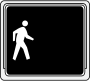
\includegraphics{MUTCD_Ped_Signal_-_Walk}}
           {\caption{Proceed into the intersection}}
\end{figure}

\begin{figure}[H]
  \fcapside
           {\includegraphics{MUTCD_Ped_Signal_-_Hand_with_timer}}
           {\caption{The walk condition will end in the indicated
               number of seconds.  Do not enter the intersection
               unless you can cross before the walk condition ends.}}
\end{figure}

\begin{figure}[H]
  \fcapside
           {\includegraphics{MUTCD_Ped_Signal_-_Steady_hand}}
           {\caption{Do not enter the intersection.}}
\end{figure}

These symbols may be accompanied by audible or tactile signals for
pedestrians with poor sight.

\subsection{Sensors}

Lanes D, H, and J do not have Traffic Approaching sensors, so their
Traffic Present sensors also set the Traffic Approaching toggles
in their respective finite state machines.

Each pedestrian crossing is equipped with a button so the pedestrian can
signal his desire to cross the street.  This is equivalent to the
Traffic Present sensor for vehicles.  When pushed it remains triggered
until the pedestrian enters the crosswalk.

\subsection{Timers}

We need additional timers to handle permissive left turns.

\subsubsection{Left Flashing Yellow Waiting Time}

Lanes A and E can allow a left turn in the presence of oncoming traffic,
called a permissive left turn. However, if oncoming traffic is heavy enough
that a waiting vehicle cannot make its turn for Left Flashing Yellow Waiting
seconds, the oncoming traffic will be stopped, thus allowing a protected left
turn.

\subsubsection{Minimum Left Flashing Yellow Time}

Once the finite state machine has turned on the left flashing yellow light
in the signal face, it keeps that light on for at least Minimum Left Flashing
Yellow seconds to make sure the left turning traffic is able to start up.

\subsubsection{Left Flashing Yellow Limit Time}

If the signal face has been showing the left flashing yellow light for
Left Flashing Yellow Limit seconds the finite state machine will turn
the signal face red even there is no conflicting traffic and there is
still traffic turning left.

\subsection{Timer Durations}

Here are the lengths of times that the timers run for.  Unlimited means
that the timer never completes; thus there is, for example, no limit on
how long signal face A can remain red.

\input {timer_durations_03.tex}

\subsection{Toggles}

This intersection has provision for manual override by a traffic control
officer.  The officer has a control panel by which he can indicate which
direction of traffic should be allowed.  Alternatively, he can set all
of the signal faces to flashing and control the traffic using hand gestures.

In addition, we need toggles to handle permissive versus protected
left turns.

\subsubsection{Flash Red}
When a malfunction or a traffic control officer sets this toggle
the finite state machine will set its signal face to flashing red.

\subsubsection{Flash Yellow}
When a malfunction or a traffic control officer sets this toggle
the finite state machine will set its signal face to flashing yellow.
Lanes A and E, which have two yellow lamps, will flash the upper lamp,
since flashing the lower lamp means that left turn is permitted.

\subsubsection{Manual Red}
When a traffic control operator sets this toggle the finite state machine
will set its signal face to red as quickly as possible consistent with
safety and keep it red until this toggle is cleared.

\subsubsection{Manual Green}
When a traffic control operator sets this toggle the finite state machine
will set its signal face to green as quickly as possible consistent with
safety and keep it green until this toggle is cleared.

\subsubsection{Request Clearance}
If a lane remains occupied after its signal face has signaled
that a permissive left turn is allowed, the finite state machine
asks that oncoming traffic also be stopped by setting toggle Request Clearance.

\subsubsection{Partial Conflicting Paths are Clear}
When a finite state machine  sees that this toggle is set
but Conflicting Paths are Clear is not set, it can
set its signal face to flashing left arrow yellow.
This can only happen for lanes A and E, since only those
finite state machines have a partial conflict table
that is different from their conflict table.

\subsection{Wiring the Finite State Machines to the Lamps}

Each finite state machine is wired to the lamps in its signal face.
This lets the signal face  use arrow lamps instead of circular lamps
to indicate to the motorist which travel paths are available to him.
Finite state machine A, for example, has its Steady Circular Red output
connected to a lamp in itsd signal face which shows a Steady Left Arrow Red.
Table \ref{lamp_map_03} shows wiring between the finite state
machines and the lamps in the signal faces.

\input {lamp_map_names_03.tex}

\subsection{Wiring the Finite State Machines to the Sensors}

Each finite state machine is wired to the sensors
for its lane.

Lanes A and E have their Traffic Approaching sensor where
the left turn lane begins; lanes B, C, F, and G have their
Traffic Approaching sensors far enough from the intersection that a vehicle
moving at the speed limit which sees the signal face turn yellow
just as he triggers the sensor has time to stop safely.

Lanes D, H, and J do not have Traffic Approaching sensors, so the output
of the Traffic Present sensor is used for both functions.

The sensors for the pedestrian crosswalks are the buttons that
the pedestrians pres to cross.

The driving public is accustomed to signal faces which control
adjacent through lanes operating together: they would think it strange
if signal face B turned red while C remained green.  We accomodate this
by connecting the sensors for lanes B and C to both finite state machines
B and C, and likewise for F and G.  We also make the timer durations
match so the pairs of finite state machines will operate in lockstep.

Similarly, if pedestrians can cross the crosswalk in one direction,
it is customary to also allow crossing in the opposite direction,
even if the sensor has not been triggered.  Thus we connect the sensors
for lanes psw and pse to both finite state machines faces psw and pse,
and the sensors for lanes pnw and pne to both finite state machines
pnw and pne.  We also make the timer durations match in finite state
machines psw and pse and also pnw and pne.

\input {sensor_map_03.tex}

\subsection{Process}

We have nine entry lanes, each with one or two sensors, plus an emergency
vehicle sensor and manual override controls.

\subsubsection{States}

Here are the full details about each state, and each substate within them.

When a signal face's finite state machine enters a particular substate
there are actions which are executed.
While it is in that substate there are conditions
that will cause it to exit the substate and enter another.

\begin{description}

\item[Red]
  The Red major state has its signal face set to red,
  which means traffic in this
  lane must stop.  When the signal face has been red for Red Clearance Time,
  the finite state machine sets its Cleared toggle, which is tested by other
  signal faces to see if they can turn green.  If a vehicle or
  pedestrian arrives at this lane it starts the process
  of turning its signal face green.

  Here are the details of the Red state:
      
  \input{red_state_table.tex}
  
\item[Green]
  The Green major state has its signal face set to green,
  which means traffic in this lane
  may proceed through the intersection.
  When the signal face light turns green
  we keep it green long enough
  for the traffic to get moving.  Afterwards if another finite state machine
  wants this one to turn red we wait for a break in the traffic.
  If there is no break in the
  traffic for a while we turn red anyway.
  If an emergency vehicle is present and not in this lane
  we turn red as quickly as we safely can.

  \input{green_state_table.tex}

\item[Yellow]
  The Yellow state is an intermediate state between green and red, and when
  flashing means that there may be conflicting traffic.  On left turn signal
  faces with a fourth light that shows a flashing yellow left arrow, that
  light is included in the Yellow state.

  \input{yellow_state_table.tex}
  
\end{description}

The State Diagram Summary in figure \ref{fig:State_Diagram_Summary}
summarizes the most significant states, substates and
transitions of the finite state machines.

\begin{figure}[htb]
  {\includegraphics{state_diagram}}
  {\caption{State Diagram Summary}\label{fig:State_Diagram_Summary}}
\end{figure}

\subsubsection{System Programs}

Communication between finite state machiness is handled by
system programs.
These system programs run constantly, reacting to toggles in the
finite state machines  by setting toggles in other finite state machines.

\begin{description}
\item [Green Request Granted]

  To prevent two finite state machines from bouncing green time between
  themselves, locking out a third finite state machine,
  this system program makes sure that
  traffic never has to wait too long for a green light.

  The Green Request Granted system program maintains a persistent list of
  finite state machines that are requesting green,
  a list of finite state machines that are allowed to turn green
  and a list of finite state machines that have turned green since the
  currently waiting signal face has had its chance.
  All of these lists start empty.

  Go through all of the finite state machines
  looking for those with toggle Request
  Green true.  Add each such finite state machines to the list of
  finite state machines that are requesting green,
  unless the finite state machine is already on
  the list or is in the list of finite state machines allowed to turn green.

  If the list of finite state machines allowed to turn green is empty, move the
  oldest finite state machine on the list of finite state machines
  that are requesting green to the list of finite state machines allowed to
  turn green and empty the list
  of finite state machines that have turned green since the currently waiting
  finite state machine has had its chance.

  Although we wish to allow the finite state machine that has been on the
  finite state machines requesting to turn green list the longest to turn green
  as soon as possible, we can let other finite state machines turn green
  at the same time or sooner if they will not delay this finite state machine
  from turning green.

  If the oldest finite state machine on the list of finite state machines
  that are requesting to turn green does not conflict with any of the
  finite state machines that are already allowed to turn green,
  move it from the list of finite state machines that are requesting
  to turn green to the list of finite state machines that are allowed
  to turn green and empty the list of finite state machines that have
  turned green since the currently waiting finite state machine has had
  its chance.

  Keep doing the above until the list is empty or the oldest finite
  state machine on the list cannot move because of a conflict.

  Now we try to let some finite state machines turn green out of order, being
  careful not to allow any other finite state machine to be starved out of any
  opportunity to turn green.

  Provided the oldest finite state machine on the list of finite state
  machines requesting to turn green has not been waiting too long,
  go through the list of finite state machines that are requesting
  to turn green starting with the oldest.
  For each such finite state machine that does not
  conflict with any of the finite state machines already in the set of
  finite state machines allowed to turn green, and is not in the list of
  finite state machines that have turned green since the currently waiting
  finite state machine has had its chance, move that finite state machine
  to the list of finite state machines allowed to turn green and add it to
  the list of finite state machines that have
  turned green since the currently waiting finite state machine has had its
  chance.

  Go through the list of finite state machines allowed to turn green.  For any
  for which toggle Traffic Flowing is true, remove them from the list
  since they have now turned green.

  Go through the list of finite state machines allowed to turn green.  For each
  such finite state machine, set its Green Request Granted toggle, telling it
  that it can now turn green.

\item[Clearance Requested]

  When a finite state machine wants to turn green,
  it must wait for all conflicting
  travel paths to become clear.  This system program conveys the request
  for clearance to the finite state machines which control entry lanes
  that conflict with this one.

  Go through all of the finite state machines looking for those with toggle
  Request Clearance true.  For each such finite state machine,
  consult the conflict table to see which lanes conflict with this one.
  For each such lane, set the Clearance Requested toggle in its finite
  state machine.

\item[Partial Clearance Requested]

  Go through all of the finite state machines looking for those with toggle
  Request Partial Clearance true.  For each such finite state machine,
  consult the partial signal face conflict table to see which lanes conflict
  with this one.  For each such lane, set the Clearance Requested toggle
  in its finite state machine.

  This is the same as Clearance Requested, but we use the partial signal face
  conflict table, which matches the conflict table except
  for the left turn lanes, where their conflict with oncoming traffic is
  omitted.
  This lets left turners try to make a permissive left turn.
  If they cannot the finite state machine will use the Clearance Requested
  toggle to cause the oncoming traffic to stop.

\item[Conflicting Paths are Clear]

  Go through the finite state machines looking for those with toggle
  Request Clearance
  or toggle Request Partial Clearance
  true.  For each such finite state machine, consult the conflict table
  to determine which entry lanes contain a travel path that conflicts
  with any of the travel paths controlled by this finite state machine's
  entry lane.  If all of the
  corresponding finite state machines have their Cleared toggles true,
  set the Conflicting Paths
  are Clear toggle in this finite state machine.

\item[Partial Conflicting Paths are Clear]

  Go through the finite state machines looking for those with toggle
  Request Partial
  Clearance true.  For each such finite state machine, consult the partial
  conflict table to determine which entry lanes contain a travel path
  that conflicts any of the travel paths controlled by this finite state
  machine's entry lane.  If all of the corresponding finite state machines
  have their Clear toggles
  true, set the Partial Conflicting Paths are Clear toggle in this
  finite state machine.

\item[Safety Check]

  Safety Check is a different kind of system program.  It does not
  monitor toggles from the various finite state machines but instead checks
  for unsafe conditions.  
  
  An error in the description of the finite state machine, or an error
  in the implementation of the finite state machine driver or the
  system programs may cause the finite state machines to get into unintended
  states, such that conflicting traffic flows are permitted in the
  intersection.  Sucn a condition is unsafe.  Check for incompatible
  states and, if such a state is found, set the intersection to flashing.

\end{description}

\subsection{Illustrations}

\subsubsection{Idle}

If there is no traffic, finite state machines A, D, E, H, J, and the
pedestrian finite state machines will remain red
since their Red Limit timers have an infinite duration; however,
finite state machines B, C, F, and G will proceed to substate
Going Green 4 when their Red Limit timers complete after 60 seconds.

In substate Going Green 4, system program Green Request Granted will notice
that finite state machines B, C, F, and G have their Request Green toggles
set.
The system program will place all four finite state machines on its list of
finite state machines requesting to turn green.
It will move one of them to the list of finite state machines allowed to
turn green.  Assume it is finite state machine B.
It will then go through finite state machines C, F, and G
and discover that finite state machine C does not have
a conflict with B and so move it to the list of finite state machines
allowed to turn green.  Similarly, finite state machine F has no conflict
with B or C, and G has no conflict with B, C, or F, so we end up with
B, C, F, and G on the list of finite state machines allowed to turn green.

Finite state machines B, C, F, and G will proceed to state Red
substate Going Green 5 where they will set toggle Request Partial Clearance.

System Program Partial Clearance Requested will notice that finite state
machines B, C, F, and G have Request Partial Clearance true,
and will consider setting toggle Clearance Requested in finite state machines
D, E, H, J, and in the pedestrian finite state machines.
However, those finite state machines
are in state Red substate Travel Path is Clear so they all have their
Cleared toggles set.

The Partial Conflicting Paths are Clear system program will notice that the
finite state machines corresponding to lanes that partially conflict with
lanes B, C, F, and G are clear, so will set the
Partial Conflicting Paths are Clear toggle in finite state machines
B, C, F, and G.
Similarly, the Conflicting Paths are Clear system program will set
the Conflicting Paths are Clear toggle in those same finite state machines.

Finite state machines B, C, F, and G will proceed from state Red substate
Going Green 5 to state Green substate No Traffic.
This will cause their signal faces to turn green and set toggle
Traffic Flowing.

System program Green Request Granted will notice that finite state machines
B, C, F, and G have their Traffic Flowing toggle true,
and so will remove them from the list of signal faces allowed to turn green.
This will cause the list to be empty.

The net effect is that after 60 seconds finite state machines
B, C, F, and G turn their signal faces green.
Because the Green Limit timer duration for these finite state machines
is unlimited the signal faces  will remain green unless
a conflicting finite state machine needs to turn green.  Because the Red Limit
timer duration for the other finite state machines is unlimited
their signal faces will stay red unless some traffic appears on their lanes.

We will call this situation, with finite state machines B, C, F, and G
in a green state and the others in a red state and clear the idle condition
for example 03, since it will persist in the absence of traffic.

This table of events details the progression from power on to the idle
condition.

\input{idle_03_table.tex}

\subsubsection{Pedestrian Crossing on South Side of Intersection}
A pedestrian at the southwest corner who wishes to cross the boulevard
presses his button.  Assuming we are in the idle condition
with finite state machines B, C, F, and G green and with A, D, E, H, J,
and the pedestrian finite state machines red and clear.

Finite state machines psw and pse will proceed through substates
Delay Green 1p and Delay Green 2p to substate
Going Green 1 where they will set toggle Request Green and
advance to substate Going Green 2.
The Green Request Granted system program will act
as described above to set the Green Request Granted toggle since no other
finite state machines are waiting to turn green.
Finite state machines psw and pse will then
proceed to substate Going Green 3 where they will set toggle Request Partial
Clearance.  System program Partial Conflicting Paths are Clear will set
the Clearance Requested toggles in finite state machines B, C, F, and G,
but not in finite state machines A, D, and J because they are aleady clear.
Finite state machines B, C, F, and G are in state Green substate
Looking for Gap 2 because their Green Limit timers have a
duration of infinity and they have seen no recent traffic.

Finite state machines B, C, F and G enter state Yellow substate Going Red.
When their Yellow Change timers complete they will proceed to state Red
substate Waiting for Clearance.
When their Red Clearance timers complete they will go
to substate Travel Path is Clear and set toggle Cleared.

The Conflicting Paths are Clear system program will notice that
finite state machines A, B, C, D, F, G, and J are all clear and set the
Conflicting Paths are Clear toggle in finite state machines psw amd pse.
Similarly, the Partial Conflicting Paths are Clear system program will set the
Partial Conflicting Paths are Clear toggle.

Finite state machines  psw and pse will transition to state Green substate
Minimum Green.
This will cause the pedestrian signal faces to display a walking man,
the equivalent of green.
Assuming there is no other traffic, finite state machines
pse and psw will remain green until the Red Limit timers complete on
finite state machines B, C, F, and G.
This will cause finite state machines pse and psw to follow the progression
described above for finite state machines B, C, F, and G.
Finite State Machines pse and psw will transition to state Yellow
substate Going Red, where they will display on their signal faces
the hand with a countdown timer showing how many seconds are left
in the Yellow Change timer.  When the Yellow Change timer is complete
finite state machines psw and pse will transition to the
Red state, substate Waiting for Clearance.  When their Red Clearance timers
completes they will transition to substate Travel Path is Clear
and set the Cleared toggle.

Signal faces B, C, F, and G will then proceed as described above
in the Idle illustration to turn their signal faces green.

The following describes these events in detail.

\input{pedestrian_table.tex}

\subsubsection{Left Turn}

A vehicle arrives at lane A.  Assume we are in the idle condition
with finite state machines B, C, F, and G green and the others red and clear.

Finite state machine A requests permission to turn green,
which it receives right away because no other finite state machine
is requesting permisison to turn green.

Finite state machine A then causes the Partial Clearance Requested system
program to set the Clearance Requested toggle in finite state machines
psw, pse, D, H, and J.

Finite state machines psw, pse, D, H, and J are already clear,
so system program Partial Conflicting Paths are Clear sets toggle
Partial Conflicting Paths are Clear in finite state machine A.
Notice that finite state machines F and G are not clear,
so toggle Conflicting Paths are Clear does not get set in
finite state machine A.

Finite state machine A proceeds to state Yellow substate Left Flashing 1.
The red light at signal face A turns to a yellow flashing light,
telling the vehicle operator that he may turn left but must watch for
oncoming traffic.

When the Minimum Left Flashing Yellow timer is completed the finite
state machine transitions to substate Left Flashing 2.

If a vehicle is still in lane A when the Left Flashing Yellow Waiting
timer completes, the finite state machine proceeds to substate
Going Green where it sets the Request Clearance toggle,
causing system program Clearance Requested to set the Clearance Requested
toggle in finite state machines psw, pse, D, F, G, H, and J.

Finite state machines psw, pse, D, H and J are already clear.
Finite state machines F and G proceed to the yellow state
and then the red state and become clear.

When finite state machines F and G become clear system program
Conflicting Paths are Clear will set the Conflicting Paths are Clear
toggle in finite state machine A which will cause signal face A to turn green.

When the Vehicle Gone timer in finite state machine A
completes, finite state machine A will proceed to state red and eventually
become clear, which will allow finite state machines F and G to turn
their signal faces green when their Red Limit timers complete,
as described above.

The following events take place assuming that the driver of the
car turning left is not willing to make the permissive turn,
and so waits for the green arrow.

\input{left_turn_delayed_table.tex}

However, if the vehicle makes the permissive left turn and there is
no further traffic, finite state machine A
returns to state red, never causing finite state machines F and G to turn
their signal faces red, as illustrated in the following events.

\input{left_turn_table.tex}

\subsubsection{Pedestrian and Near Left Turner}

Building upon the previous two illustrations, suppose after the pedestrian
has pushed his button and begun to cross, a vehicle arrives at lane A.
Finite state machine A will be be given permission to turn green right away,
since no other finite state machines are waiting to turn green.
It will then request that finite state machines psw, pse, D, H, and J
turn red.  Finite state machines D and J
will already be clear because of the previous request by finite state
machines pse and psw.
Finite state machine H has never been green so finite state machine A
is waiting only for finite state machines psw and pse.

When the pedestrian finishes crossing and finite state machines
psw and pse are clear finite state machine A will turn its signal face
left arrow green rather than flashing left arrow yellow because
finite state machines F and G are clear due to the previous request
by finite state machines psw and pse,
so the left turn is protected rather than permissive.

Finite state machines B, C, F, and G will eventually want to turn green
and so finite state machines F and G will ask finite state machine
A to turn red.  Finite state machines B and C
will turn green without waiting for finite state machine A to clear, since
they do not conflict.  When finite state machine A is clear finite state
machines F and G will turn green, getting us back to the idle state.

Here are the events of this illustration.

\input{pedestrian_and_left_turn_table.tex}

Here is an animation, which provides the same illustration in graphic form.

\noindent\includemedia[width=\textwidth,
  addresource=pedestrian_and_left_turn_animation_03.mkv,
  activate=onclick, attachfiles,
  flashvars={source=pedestrian_and_left_turn_animation_03.mkv &loop=false}
]{{\includegraphics[width=\textwidth]{background_03}}}{VPlayer.swf}

If your PDF viewer will not play the animation you can see it on Youtube
by navigating to URL \href%
{https://www.youtube.com/playlist?list=PLCGHQeqDmNySa8JSIUioGNoWbXebCGjyx}%
{https://www.youtube.com/playlist?list=PLCGHQeqDmNySa8JSIUioGNoWbXebCGjyx}
and choosing pedestrian and left turn animation 03.

\subsubsection{Multiple Arrivals}

Suppose we are in the idle condition when traffic arrives in quick succession
on lanes A, psw, D, E, pne, H, and J in that order.

Finite state machine A turns left flashing yellow immediately since lanes
F and G are allowing traffic to flow.

Finite state machine psw asks finite state machines A, B, C, F, and G to
turn red.
Finite state machine A is currently left flashing yellow but finite state
machines B, C, F, and G turn yellow and then red.

With the through lanes all stopped finite state machine face A turns
green, then yellow, then red, permitting the pedestrian in the south
crosswalk to cross.  Signal face E does the same, permitting first its
own vehicle and then the
pedestrian in the north crosswalk to cross.  The lane E vehicle and
the pedestrian on the north crosswalk are allowed
to enter the intersection out of turn because they can enter the
intersection at the same time as the pedestrian crossing the south crosswalk.

When the pedestrian in the south crosswalkhas crossed, finite state machine
J turns green.  Similarly, when the pedestrian in the
north crosswalk have crossed, finite state machine H turns green.

When finite state machines H and J have turned red, signal face D
can finally turn green.  When it turns red signal faces
B, C, F, and G turn green, getting us back to the idle state.

To summarize, if traffic arrives in quick succession on signal faces
A, psw, D, E, pne, H and J, traffic will flow through signal faces
A and E, then through psw and pne, then H and J, and finally D.

The following table shows the most significant events in this scenario.

\input{multiple_table.tex}

Here is an animation of the multiple arrivals scenario:

\noindent\includemedia[width=\textwidth,
  addresource=multiple_animation_03.mkv,
  activate=onclick, attachfiles,
  flashvars={source=multiple_animation_03.mkv &loop=false}
]{{\includegraphics[width=\textwidth]{background_03}}}{VPlayer.swf}

If your PDF viewer will not play the animation you can see it on Youtube
by navigating to URL \href%
{https://www.youtube.com/playlist?list=PLCGHQeqDmNySa8JSIUioGNoWbXebCGjyx}%
{https://www.youtube.com/playlist?list=PLCGHQeqDmNySa8JSIUioGNoWbXebCGjyx}
and choosing multiple animation 03.

There are other animations in that playlist which further illustrate
how traffic control signals handle traffic.

\section{Manual Control}

An operator may take manual control of the traffic control signal.
The operator's control panel contains the following controls:

\subsection{Off Switch}
The Off switch turns off power to the traffic control signal and all
of the signal faces.  Turning off power is necessary for safety during
maintenance.

\subsection{Mode}

There is a multi-position mode switch:

\subsubsection{Automatic}

With the mode switch set to Automatic the traffic control signal
processes signals from the sensors and acts appropriately, as described
above.  The operator is an observer who can see the color of each
signal face, the state of each vehicle detector,
and the names of the finite state machines in each persistent list
maintained by the Green Request Granted system program.

The operator can choose to also see the state and substate of each
finite state machine, the condition of each timer, the time until completion
of each running timer, and the condiiton of each toggle.

\subsubsection{Manual}

With the mode switch set to Manual, the traffic control signal is
not responsive to the sensors.  The operator has
a 3-position switch on the display of each lane to cause that lane to turn red
or green.  The Red position sets the Manual
Red sensor, the green position sets the Manual Green sensor, and
the third position is neutral, which sets neither sensor.

In this mode, as in Automatic mode, the operator sees the color of
each signal face and the state of each vehicle sensor.
Also as in Automatic mode,
the operator can choose to also see the state and substate of each
finite state machine, the condition of each timer, the time until completion
of each running timer, and the condition of each toggle.

In this mode the operator must manually turn each signal face
red and green using his 3-position switches.  Setting all of the switches
to neutral is equivalnet to automatic mode.

Notice that all of the safety interlocks still
are in effect: setting a finite state machine's Manual Green sensor
while a conflicting finite state machine is in the green state
because its Manual Green toggle is set will have no effect until the
operator sets the conflicting signal faces to red or neutral.
There are options in the manual control panel to automatically set all
conflicting signal faces to red or to neutral when a signal face
is manually set to green.  There are also options to group lanes
together so that moving one switch changes toggles in
more than one finite state machine.

A manual control panel can be either local or remote.  If it is remote
there should be cameras giving a complete picture of the intersection
to the remote operator.

\subsubsection{Flashing}

With the mode switch set to Flashing, each finite state machine will
turn red or yellow as quickly as possible consistent with safety, and then
flash its signal face either red or yellow.

If the traffic signal controller detects an internal malfunction it switches
all of the finite state machines to Flashing mode.
In addition, if the computer in the traffic
signal controller fails there is hardware in the traffic signal
controller to flash the lights independent of the computer,
though in this case it will not be possible to first turn the
signal face red or yellow safely.

\subsubsection{Programming}

This mode is protected so only authorized persons can access it.
It works the same as Automatic mode except the operator is also allowed to
adjust the duration of the timers in each finite state machine, and update the
Conflict Table and the Partial Conflict Table.

These adjustments can cause unsafe conditions and so should be limited
to highly trusted personnel.

\section{Central Control}

The signaling procedure described here takes only the traffic at a single
intersection into account.  Where there are many intersections close
together it will be worthwhile to control them all as a single system.
In such a control system a central controller will provide overall
coordination while each intersecton operates as described here except as
directed by the central controller.

The algorithm used by the central controller is beyond the scope of this
description, but from the point of view of an individual intersection
the central controller will use the Manual Green toggle to clear paths
through several intersections so that traffic can flow freely in the
chosen directions.

The central controller will be able to see all of the sensors of all
of the intersections it controls and will be able to watch all of
the traffic through cameras.

As an alternative to a central controller some coordination between
intersections can be achieved by connecting the sensors of one intersection
to the Traffic Approaching toggles of downstream intersections.

\section{More Details}

If you would like more details about how a traffic control signal works,
you can examine the software used to prepare the tables and animations
for this paper.  The software is on github at this URL:

\href{https://github.com/JohnSauter/How\_Traffic\_Control\_Signals\_Work}{https://github.com/JohnSauter/How\_Traffic\_Control\_Signals\_Work}

That github repository includes a spec file to facilitate building
this paper using COPR.  That spec file is also included in the tarball.

\section{Licensing}
\label{section:Licensing}
As noted on the first page, this paper is licensed under a Creative
Commons Attribution-ShareAlike 4.0 International License.

The full text of the Creative Commons Attribution-ShareAlike 4.0
International license is at this web site:
\href{https://creativecommons.org/licenses/by-sa/4.0/legalcode}{https://creativecommons.org/licenses/by-sa/4.0/legalcode}
What follows is a human-readable summary of it.

\subsection{You are free to:}
\begin{description}
\item[Share ---]copy and redistribute the material in any medium or format, and
\item[Adapt ---]remix, transform, and build upon the material
\end{description}
for any purpose, even commercially.  The licensor cannot revoke these
freedoms as long as you follow the license terms.
\subsection{Under the following terms:}
\begin{description}
\item[Attribution ---]You must give appropriate credit\footnote{If supplied,
  you must provide the name of the creator and attribution parties,
  a copyright notice, a license notice, a disclaimer notice, and a link
  to the material.}, provide a link to
  the license, and indicate if changes were made\footnote{You must indicate if
    you modified the material and retain an indication of previous
    modifications.}.  You may do so in any
  reasonable manner, but not in any that suggests the licensor endorses you
  or your use.
\item[ShareAlike ---]If you remix, transform, or build upon the material,
  you must distribute your contributions under the same
  license\footnote{You may also use any of the licenses listed as compatible
    at the following web site:
    \href{https://creativecommons.org/compatiblelicenses}{https://creativecommons.org/compatiblelicenses}}
  as the original.
\item[No additional restrictions ---]You may not apply legal terms or
  technological measures\footnote{The license prohibits application of
    effective technological measures, defined with reference to Article 11
    of the WIPO Copyright Treaty.}
  that legally restrict others from doing anything
  the license permits.
\end{description}
\subsection{Notices:}
\begin{itemize}
\item{You do not have to comply with the license for elements of the
  material in the public domain or where your use is permitted by an
  exception or limitation.}
\item{No warranties are given.  The license may not give you all of the
  permissions necessary for your intended use.  For example, other rights
  such as publicity, privacy or moral rights may limit how you use the
  material.}
\end{itemize}

\bibliography{references}

\end{document}
